\section{MINAS}
\label{sec:minas}

%  ******************* Texto quali ************************
% \subsection{O Algoritmo MINAS}
% Apresentar o MINAS de forma resumida (1 pagina no max): como funciona, etc. 

\minas \cite{Faria2013Minas,Faria2015minas} is an offline-online \nd algorithm,
meaning it has two distinct phases. The first phase (offline) creates a initial
model set with several clusters based on a clustering algorithm with a training
set.
Each cluster can be associated with only one class of the problem, but each
class can have many clusters.

The online phase is where the model performs three tasks in (near) real-time.
% Our proposal focuses on the online phase, therefore we will describe it in more detail.
We describe the online phase in more detail since we focus on its tasks.
In summary, the online phase of \minas executes classification, novelty
detection, and model update tasks until the possible end of stream, as shown in
Algorithm \ref{alg:MINAS}.
\minas tries to classify each incoming unlabeled instance according to the
current decision model. Instances not explained by the current model
receive an \textit{unknown} label and are stored in the unknowns-buffer.
When the unknowns-buffer reaches a parametric size, \minas executes the
Novelty Detection function.
Beyond the Novelty Detection, \minas also cleans the unknowns-buffer removing
old instances as they represent noise or outliers and, has a mechanism to forget
clusters that became obsolete and unrepresentative of the current data stream
distribution \cite{Faria2015minas}.

\begin{algorithm}
    % \DontPrintSemicolon
    \SetKwFunction{nearestCluster}{nearestCluster}
    \SetKwFunction{clustering}{clustering}
    \SetKwFunction{NoveltyDetection}{NoveltyDetection}
    \SetKwFunction{handleModelSleep}{moveToSleep}
    \SetKwFunction{removeOldSamples}{removeOldSamples}
    % 
    \SetKwProg{Function}{Function}{:}{}
    \SetKwFor{With}{with}{}{}
    \SetKw{continue}{continue}
    % 
    \KwIn{ModelSet, inputStream}
    \KwOut{outputStream}
    % 
    \SetKwData{cleaningWindow}{cleaningWindow}
    \SetKwData{noveltyDetectionTrigger}{noveltyDetectionTrigger}
    \SetKwInOut{KwParams}{Parameters}
    \KwParams{\cleaningWindow, \noveltyDetectionTrigger}
    % \KwSty{Parameters}: \cleaningWindow, \noveltyDetectionTrigger\\
    % 
    \SetKwFunction{MinasOnline}{MinasOnline}
    \Function{\MinasOnline{ModelSet, inputStream}}{
        UnkownSet $\leftarrow$ $\emptyset$, ModelSleepSet $\leftarrow$ $\emptyset$ \;
        lastCleanup $\leftarrow 0$ , noveltyIndex $\leftarrow 0$\;
        % sampleIn $\leftarrow 0$\;
        \ForEach{ {$sample_{i}$} $\in$ inputStream }{
            % sample.label $\leftarrow$ unknown\;
            % (distance, cluster) $\leftarrow$ \nearestCluster(sample, ModelSet)\;
            nearest $\leftarrow$ \nearestCluster(sample, ModelSet)\;
            \eIf{nearest.distance $<$ nearest.cluster.radius}{
                sample.label $\leftarrow$ nearest.cluster.label\;
                nearest.cluster.lastUsed $ \leftarrow i $ \;
            }
            {
                sample.label $\leftarrow$ unknown\;
                UnkownSet $\leftarrow$ UnkownSet $\cup$ sample\;
                \If{$|\;UnkownSet\;| \geq$ \noveltyDetectionTrigger}{
                    % \tcc{Novelty Detection}
                    novelties $\leftarrow$ \NoveltyDetection(ModelSet $\cup$ ModelSleepSet, *UnkownSet)\;
                    ModelSet $\leftarrow$ ModelSet $\cup$ novelties\;
                }
                \If{ $ i > $ ( lastCleanup $ + $ \cleaningWindow )}{
                    ModelSet $\leftarrow$ \handleModelSleep(ModelSet, *ModelSleepSet, lastCleanup)\;
                    UnkownSet $\leftarrow$ \removeOldSamples(UnkownSet, lastCleanup)\;
                    lastCleanup $ \leftarrow i $\;
                }
            }
            outputStream.append(sample)\;
        }
    }
\label{alg:MINAS}
\caption{Our interpretation of \minas \cite{Faria2015minas}}
\end{algorithm}

The Novelty Detection function, shown in Algorithm \ref{alg:MINAS-nd} groups the
instances to form new clusters and each new cluster is validated to discard the
non-cohesive or unrepresentative ones.
Valid clusters are analyzed to decide if they represent an extension of a
known pattern or a completely new pattern. In both cases, the model absorbs the
valid clusters and starts using them to classify new instances.

\begin{algorithm}[h]
    \SetKwProg{Function}{Function}{:}{}
    \SetKwData{minExamplesPerCluster}{minExamplesPerCluster}
    \SetKwData{noveltyFactor}{noveltyFactor}
    \SetKwInOut{KwParams}{Parameters}
    \KwParams{\minExamplesPerCluster, \noveltyFactor}
    % 
    \SetKwFunction{nearestCluster}{nearestCluster}
    \SetKwFunction{clustering}{clustering}
    \SetKwFunction{NoveltyDetection}{NoveltyDetection}
    \SetKwFunction{handleModelSleep}{moveToSleep}
    \SetKwFunction{removeOldSamples}{removeOldSamples}
    % 
    \Function{\NoveltyDetection{Model, Unknowns}}{
        newModelSet $\leftarrow$ $\emptyset$\;
        \ForEach{cl in \clustering(Unknowns)}{
            \If{$|\;cl.sampleSet\;| \geq$ \minExamplesPerCluster}{
                (distance, near) $\leftarrow$ \nearestCluster(cl, Model)\;
                \eIf{distance $<$ near.radius $\times$ \noveltyFactor}{
                    cl.label $\leftarrow$ near.label\;
                    cl.type $\leftarrow$ extension\;
                }{
                    cl.label $\leftarrow$ noveltyIndex\;
                    noveltyIndex $\leftarrow$ noveltyIndex $+ 1$\;
                    cl.type $\leftarrow$ novelty\;
                }
                \label{alg:MINAS-nd:reclassify}
                Unknowns $\leftarrow$ Unknowns $-$ cl.sampleSet\;
                newModelSet $\leftarrow$ newModelSet $\cup$ cl\;
            }
        }
        \Return{newModelSet}\;
    }
    \label{alg:MINAS-nd}
    \caption{\minas \cite{Faria2015minas} Novelty Detection task.}
\end{algorithm}


% Citar que o trabalho anterior já validou o uso do MINAs para detecção de novidade porem com uma implementação sequencial. 

% Authors in~\cite{Cassales2019a} validated the usage of the MINAS algorithm for
% the Intrusion Detection and deploying it on edge. However, they used the
% sequential version of the algorithm, where classification stops completely to
% execute novelty detection.

% Figura do MINAS (offline + online) ...
% \todo[inline, color=brown]{\textbf{Guilherme:} Não coloquei figura porque as figuras originais do MINAS ocupam bastante espaço (https://sci-hub.se/10.1007/s10618-015-0433-y pg 9) e a do MFog está mais completa.}

% Formally, a data stream $S$ is a massive sequence of data elements
% $x_1, x_2, \dots, x_n$ that is, $S={\{x_i\}}_{i=1}^n$, which is potentially
% unbounded (n → $\infty$).
% Compared to traditional (batch) data mining, stream processing algorithms have
% additional requirements.
% For instance, with a potentially infinite data stream, storing data for late
% processing is not a choice due to memory constraints.
% Algorithms need to incrementally process incoming data instances in a single
% pass while operating under memory and response time constraints.
% Furthermore, as data streams present transient behavior, prediction models often
% need to be incremented to adapt to concept drift observed in data.


% 
% \begin{algorithm}
%     \DontPrintSemicolon
%     \SetKwFunction{FMain}{Main}
%     \SetKwProg{Fn}{algorithm}{:}{}
%     \Fn{\FMain{$f$, $a$, $b$, $\varepsilon$}}{
%           a\;
%           b\;
%           \KwRet\;
%     }
%     \;
%     \SetKwProg{Pn}{algorithm}{:}{\KwRet}
%     \Pn{\FMain{$f$, $a$, $b$, $\varepsilon$}}{
%           a\;
%           b\;
%     }
% \end{algorithm}
% \IncMargin{1em}
\begin{algorithm}[h]

% \begin{multicols}{2}
    \SetKwProg{Function}{Function}{:}{}
    % \DontPrintSemicolon
    % \KwIn{sample, ModelSet, params as p}
    % \KwOut{Classified Sample}
    % 
    \SetKwData{CW}{cleaningWindow}
    \SetKwData{NDT}{noveltyDetectionTrigger}
    \SetKwData{MEPC}{minExamplesPerCluster}
    \SetKwData{NF}{noveltyFactor}
    % 
    % \KwSty{Parameters}: cleaningWindow as \CW,
    % noveltyDetectionTrigger as \NDT,
    % minExamplesPerCluster as \MEPC,
    % noveltyFactor as \NF\\
    % 
    \SetKwFunction{nearestCluster}{nearestCluster}
    \SetKwFunction{clustering}{clustering}
    \SetKwFunction{sizeOf}{sizeOf}
    \SetKwFunction{NoveltyDetection}{NoveltyDetection}
    \SetKwFunction{handleModelSleep}{moveToSleep}
    \SetKwFunction{removeOldSamples}{removeOldSamples}
    % 
    % \KwData{ UnkownSet $\leftarrow$ $\emptyset$, ModelSleepSet $\leftarrow$ $\emptyset$, lastCleanupTime $\leftarrow$ now() }
    % 
    \Function{\NoveltyDetection{Model, Samples}}{
        newModelSet $\leftarrow$ $\emptyset$\;
        \ForEach{cl in \clustering(Samples)}{
            \If{$|cl.sampleSet| \geq$ \MEPC}{
                (distance, near) $\leftarrow$ \nearestCluster(cl, Model)\;
                \eIf{distance $<$ near.radius $\times$ \NF}{
                    cl.label $\leftarrow$ near.label\;
                    cl.type $\leftarrow$ extension\;
                }{
                    cl.label $\leftarrow$ noveltyIndex\;
                    noveltyIndex $\leftarrow$ noveltyIndex $+ 1$\;
                    cl.type $\leftarrow$ novelty\;
                }
                Samples $\leftarrow$ Samples $\ominus$ cl.sampleSet\;
                newModelSet $\leftarrow$ newModelSet $\oplus$ cl\;
            }
        }
        \Return{newModelSet}
    }
    \label{alg:MINAS-nd}
    \caption{Minas: Novelty Detection task.}
\end{algorithm}
\begin{algorithm}
    \SetKwProg{function}{Function}{:}{}
    % \DontPrintSemicolon
    % \KwIn{sample, ModelSet, params as p}
    % \KwOut{Classified Sample}
    % 
    \SetKwData{CW}{cleaningWindow}
    \SetKwData{NDT}{noveltyDetectionTrigger}
    \SetKwData{MEPC}{minExamplesPerCluster}
    \SetKwData{NF}{noveltyFactor}
    % 
    % \KwSty{Parameters}: cleaningWindow as \CW,
    % noveltyDetectionTrigger as \NDT,
    % minExamplesPerCluster as \MEPC,
    % noveltyFactor as \NF\\
    % 
    \SetKwFunction{nearestCluster}{nearestCluster}
    \SetKwFunction{clustering}{clustering}
    \SetKwFunction{sizeOf}{sizeOf}
    \SetKwFunction{NoveltyDetection}{NoveltyDetection}
    \SetKwFunction{handleModelSleep}{moveToSleep}
    \SetKwFunction{removeOldSamples}{removeOldSamples}
    % 
    \SetKwProg{algorithm}{algorithm}{:}{}
    \SetKwFor{With}{with}{}{}
    \SetKw{continue}{continue}
    % 
    \SetKwData{CW}{CW}
    \SetKwData{noveltyDetectionTrigger}{NDT}
    \SetKwData{MEPC}{MEPC}
    \SetKwData{NF}{NF}
    \SetKwData{mpiSize}{mpiSize}
    \SetKwData{mpiRank}{mpiRank}
    \SetKwData{EndOfStream}{EndOfStream}
    % 
    \KwIn{ModelSet, Sample Stream}
    \KwOut{Classified Stream as $out$}
    \SetKwFunction{MinasOnline}{MinasOnline}
    \function{\MinasOnline{ModelSet, SampleStream}}{
        UnkownSet $\leftarrow$ $\emptyset$, ModelSleepSet $\leftarrow$ $\emptyset$ \;
        lastCleanup $\leftarrow 0$ , noveltyIndex $\leftarrow 0$\;
        % sampleIn $\leftarrow 0$\;
        \ForEach{ {$sample_{i}$} $\in$ SampleStream }{
            % sample.label $\leftarrow$ unknown\;
            % (distance, cluster) $\leftarrow$ \nearestCluster(sample, ModelSet)\;
            nearest $\leftarrow$ \nearestCluster(sample, ModelSet)\;
            \eIf{nearest.distance $<$ nearest.cluster.radius}{
                sample.label $\leftarrow$ nearest.cluster.label\;
                nearest.cluster.lastUsed $ \leftarrow i $ \;
                % $out \leftarrow$ sample\;
                % outputStream.append(sample);
                % \textbf{continue};
                % \Return sample\;
            }
            {
                sample.label $\leftarrow$ unknown\;
                UnkownSet $\leftarrow$ UnkownSet $\cup$ sample\;
                \If{$|UnkownSet| \geq$ \NDT}{
                    % \tcc{Novelty Detection}
                    novelties $\leftarrow$ \NoveltyDetection(ModelSet $\cup$ ModelSleepSet, *UnkownSet)\;
                    ModelSet $\leftarrow$ ModelSet $\cup$ novelties\;
                }
                \If{ $ i > $ ( lastCleanup $ + $ \CW )}{
                    ModelSet $\leftarrow$ \handleModelSleep(ModelSet, *ModelSleepSet, lastCleanup)\;
                    UnkownSet $\leftarrow$ \removeOldSamples(UnkownSet, lastCleanup)\;
                    lastCleanup $ \leftarrow i $\;
                }
                % \Return sample\;
            }
            outputStream.append(sample);
            % $out \leftarrow$ sample\;
        }
    }
% \end{multicols}
% }
\label{alg:MINAS}
\caption{Our interpretation of MINAS \cite{faria2013novelty,Faria2016minas,Cassales2019a}}
\end{algorithm}
% \DecMargin{1em}


% --------------------------------------------------------------------------------------------------

% \begin{algorithm}[ht]
%   \caption{MINAS \cite{Faria2016minas,Cassales2019a}}
%   \label{alg:MINAS}
%   \renewcommand{\algorithmicrequire}{\textbf{Entrada:}}
%   \begin{algorithmic}[1]
%     %T $\leftarrow$ limiar de distância para pertencer ao grupo
%     %P $\leftarrow$ tempo de "inatividade" para passar para memória sleep
%     %ts $\leftarrow$ limiar para remoção de exemplos da memória temporária
%     \REQUIRE $Modelo,FCD,T,NumMinExemplos,ts,P$
%     \STATE $MemTmp \leftarrow \emptyset$
%     \STATE $MemSleep \leftarrow \emptyset$
%     \FORALL{$exemplo \in FCD$}
%     \STATE $(Dist,micro) \leftarrow$ micro-mais-proximo($exemplo,Modelo$)
%     \IF{$Dist < $ raio($micro$)}
%     \STATE $exemplo.classe \leftarrow micro.rotulo$
%     \STATE atualizar-micro($micro,exemplo$)
%     \ELSE
%     \STATE $exemplo.classe \leftarrow desconhecido$
%     \STATE $MemTmp \leftarrow MemTmp \cup exemplo$
%     \IF{$|MemTmp| \geq NumMinExemplos$}
%     \STATE $Modelo \leftarrow $ deteccao-novidade($Modelo,MemTmp,T$)
%     \ENDIF
%     \ENDIF
%     \STATE $TempoAtual \leftarrow exemplo.T$
%     \IF{$TempoAtual$ mod $TamJanela == 0$}
%     \STATE $Modelo \leftarrow$ mover-micro-grupos-mem-sleep($Modelo,MemSleep,P$)
%     \STATE $MemTmp \leftarrow$ remover-exemplos-antigos($MemTmp,ts$)
%     \ENDIF
%     \ENDFOR
%   \end{algorithmic}
% \end{algorithm}

% \begin{algorithm}[ht]
%   \caption{MINAS \cite{Faria2016minas,Cassales2019a}}
%   \label{alg:MINAS}
%   \renewcommand{\algorithmicrequire}{\textbf{Entrada:}}
%   \begin{algorithmic}[1]
%   \IF{root}
%     \WHILE{true}
%     \IF{can_read(S)}
%     input(S, $s$)
%     send(s, i++)
%     \ENDIF
%     \IF{can_rcv($(s, l)$, any)}
%         output($(s, l)$)
%         \IF{$l == '-'$ )}
%             store($(s, l)$, unknowns)
%             % \IF{$|MemTmp| \geq NumMinExemplos$}
%             % \STATE $Modelo \leftarrow $ deteccao-novidade($Modelo,MemTmp,T$)
%             % \ENDIF
%             % \ENDIF
%             % \STATE $TempoAtual \leftarrow exemplo.T$
%             % \IF{$TempoAtual$ mod $TamJanela == 0$}
%             % \STATE $Modelo \leftarrow$ mover-micro-grupos-mem-sleep($Modelo,MemSleep,P$)
%             % \STATE $MemTmp \leftarrow$ remover-exemplos-antigos($MemTmp,ts$)
%             % \ENDIF
%         \ENDIF
%     \ENDIF
%   \ENDWHILE
%   \ENDIF
%   \IF{leaf}
%     rcv($s$, root)
%     $l$ $\leftarrow$ classify($s$)
%     send($(s, l)$, root)
%   \ENDIF
%   \end{algorithmic}
% \end{algorithm}

% \begin{algorithm}
%   \caption{High level parallel algorithm}
%   \label{alg:highlevel-new}
%   \begin{algorithmic}[1]
%     \State {\bf Input}: an ensemble $E$, $num\_threads$, a data stream $S$
%     \State $P \gets Create\_service\_thread\_pool(num\_threads)$
%     \State $T \gets Create\_trainers\_collection(E)$
%     \For {each arriving instance $I$ in stream $S$}
%     \State $E$.classify($I$)
%     \For  {each trainer $T_i$ in trainers $T$} 
%     \State $k \gets poisson(\lambda)$
%     \State $T_i.update(I, k)$
%     \EndFor
%     \For {all trainers $T$} {\bf in parallel}
%     \State $W\_inst \gets I * k$
%     \State $Train\_on\_instance(W\_inst)$
%     \EndFor
%     \If {change detected}
%     \State $reset\_classifier$
%     \EndIf
%     \EndFor
%   \end{algorithmic}
% \end{algorithm}



% \begin{figure}[ht]
% \subfloat[float]{
% \begin{minipage}[c][1\width]{0.5\textwidth}
%     \begin{algorithm}[h]
%     % {\tiny 
% \begin{algorithm}
%     \DontPrintSemicolon
%     \SetKwFunction{FMain}{Main}
%     \SetKwProg{Fn}{algorithm}{:}{}
%     \Fn{\FMain{$f$, $a$, $b$, $\varepsilon$}}{
%           a\;
%           b\;
%           \KwRet\;
%     }
%     \;
%     \SetKwProg{Pn}{algorithm}{:}{\KwRet}
%     \Pn{\FMain{$f$, $a$, $b$, $\varepsilon$}}{
%           a\;
%           b\;
%     }
% \end{algorithm}
% \IncMargin{1em}
\begin{algorithm}[h]

% \begin{multicols}{2}
    \SetKwProg{Function}{Function}{:}{}
    % \DontPrintSemicolon
    % \KwIn{sample, ModelSet, params as p}
    % \KwOut{Classified Sample}
    % 
    \SetKwData{CW}{cleaningWindow}
    \SetKwData{NDT}{noveltyDetectionTrigger}
    \SetKwData{MEPC}{minExamplesPerCluster}
    \SetKwData{NF}{noveltyFactor}
    % 
    % \KwSty{Parameters}: cleaningWindow as \CW,
    % noveltyDetectionTrigger as \NDT,
    % minExamplesPerCluster as \MEPC,
    % noveltyFactor as \NF\\
    % 
    \SetKwFunction{nearestCluster}{nearestCluster}
    \SetKwFunction{clustering}{clustering}
    \SetKwFunction{sizeOf}{sizeOf}
    \SetKwFunction{NoveltyDetection}{NoveltyDetection}
    \SetKwFunction{handleModelSleep}{moveToSleep}
    \SetKwFunction{removeOldSamples}{removeOldSamples}
    % 
    % \KwData{ UnkownSet $\leftarrow$ $\emptyset$, ModelSleepSet $\leftarrow$ $\emptyset$, lastCleanupTime $\leftarrow$ now() }
    % 
    \Function{\NoveltyDetection{Model, Samples}}{
        newModelSet $\leftarrow$ $\emptyset$\;
        \ForEach{cl in \clustering(Samples)}{
            \If{$|cl.sampleSet| \geq$ \MEPC}{
                (distance, near) $\leftarrow$ \nearestCluster(cl, Model)\;
                \eIf{distance $<$ near.radius $\times$ \NF}{
                    cl.label $\leftarrow$ near.label\;
                    cl.type $\leftarrow$ extension\;
                }{
                    cl.label $\leftarrow$ noveltyIndex\;
                    noveltyIndex $\leftarrow$ noveltyIndex $+ 1$\;
                    cl.type $\leftarrow$ novelty\;
                }
                Samples $\leftarrow$ Samples $\ominus$ cl.sampleSet\;
                newModelSet $\leftarrow$ newModelSet $\oplus$ cl\;
            }
        }
        \Return{newModelSet}
    }
    \label{alg:MINAS-nd}
    \caption{Minas: Novelty Detection task.}
\end{algorithm}
\begin{algorithm}
    \SetKwProg{function}{Function}{:}{}
    % \DontPrintSemicolon
    % \KwIn{sample, ModelSet, params as p}
    % \KwOut{Classified Sample}
    % 
    \SetKwData{CW}{cleaningWindow}
    \SetKwData{NDT}{noveltyDetectionTrigger}
    \SetKwData{MEPC}{minExamplesPerCluster}
    \SetKwData{NF}{noveltyFactor}
    % 
    % \KwSty{Parameters}: cleaningWindow as \CW,
    % noveltyDetectionTrigger as \NDT,
    % minExamplesPerCluster as \MEPC,
    % noveltyFactor as \NF\\
    % 
    \SetKwFunction{nearestCluster}{nearestCluster}
    \SetKwFunction{clustering}{clustering}
    \SetKwFunction{sizeOf}{sizeOf}
    \SetKwFunction{NoveltyDetection}{NoveltyDetection}
    \SetKwFunction{handleModelSleep}{moveToSleep}
    \SetKwFunction{removeOldSamples}{removeOldSamples}
    % 
    \SetKwProg{algorithm}{algorithm}{:}{}
    \SetKwFor{With}{with}{}{}
    \SetKw{continue}{continue}
    % 
    \SetKwData{CW}{CW}
    \SetKwData{noveltyDetectionTrigger}{NDT}
    \SetKwData{MEPC}{MEPC}
    \SetKwData{NF}{NF}
    \SetKwData{mpiSize}{mpiSize}
    \SetKwData{mpiRank}{mpiRank}
    \SetKwData{EndOfStream}{EndOfStream}
    % 
    \KwIn{ModelSet, Sample Stream}
    \KwOut{Classified Stream as $out$}
    \SetKwFunction{MinasOnline}{MinasOnline}
    \function{\MinasOnline{ModelSet, SampleStream}}{
        UnkownSet $\leftarrow$ $\emptyset$, ModelSleepSet $\leftarrow$ $\emptyset$ \;
        lastCleanup $\leftarrow 0$ , noveltyIndex $\leftarrow 0$\;
        % sampleIn $\leftarrow 0$\;
        \ForEach{ {$sample_{i}$} $\in$ SampleStream }{
            % sample.label $\leftarrow$ unknown\;
            % (distance, cluster) $\leftarrow$ \nearestCluster(sample, ModelSet)\;
            nearest $\leftarrow$ \nearestCluster(sample, ModelSet)\;
            \eIf{nearest.distance $<$ nearest.cluster.radius}{
                sample.label $\leftarrow$ nearest.cluster.label\;
                nearest.cluster.lastUsed $ \leftarrow i $ \;
                % $out \leftarrow$ sample\;
                % outputStream.append(sample);
                % \textbf{continue};
                % \Return sample\;
            }
            {
                sample.label $\leftarrow$ unknown\;
                UnkownSet $\leftarrow$ UnkownSet $\cup$ sample\;
                \If{$|UnkownSet| \geq$ \NDT}{
                    % \tcc{Novelty Detection}
                    novelties $\leftarrow$ \NoveltyDetection(ModelSet $\cup$ ModelSleepSet, *UnkownSet)\;
                    ModelSet $\leftarrow$ ModelSet $\cup$ novelties\;
                }
                \If{ $ i > $ ( lastCleanup $ + $ \CW )}{
                    ModelSet $\leftarrow$ \handleModelSleep(ModelSet, *ModelSleepSet, lastCleanup)\;
                    UnkownSet $\leftarrow$ \removeOldSamples(UnkownSet, lastCleanup)\;
                    lastCleanup $ \leftarrow i $\;
                }
                % \Return sample\;
            }
            outputStream.append(sample);
            % $out \leftarrow$ sample\;
        }
    }
% \end{multicols}
% }
\label{alg:MINAS}
\caption{Our interpretation of MINAS \cite{faria2013novelty,Faria2016minas,Cassales2019a}}
\end{algorithm}
% \DecMargin{1em}


% --------------------------------------------------------------------------------------------------

% \begin{algorithm}[ht]
%   \caption{MINAS \cite{Faria2016minas,Cassales2019a}}
%   \label{alg:MINAS}
%   \renewcommand{\algorithmicrequire}{\textbf{Entrada:}}
%   \begin{algorithmic}[1]
%     %T $\leftarrow$ limiar de distância para pertencer ao grupo
%     %P $\leftarrow$ tempo de "inatividade" para passar para memória sleep
%     %ts $\leftarrow$ limiar para remoção de exemplos da memória temporária
%     \REQUIRE $Modelo,FCD,T,NumMinExemplos,ts,P$
%     \STATE $MemTmp \leftarrow \emptyset$
%     \STATE $MemSleep \leftarrow \emptyset$
%     \FORALL{$exemplo \in FCD$}
%     \STATE $(Dist,micro) \leftarrow$ micro-mais-proximo($exemplo,Modelo$)
%     \IF{$Dist < $ raio($micro$)}
%     \STATE $exemplo.classe \leftarrow micro.rotulo$
%     \STATE atualizar-micro($micro,exemplo$)
%     \ELSE
%     \STATE $exemplo.classe \leftarrow desconhecido$
%     \STATE $MemTmp \leftarrow MemTmp \cup exemplo$
%     \IF{$|MemTmp| \geq NumMinExemplos$}
%     \STATE $Modelo \leftarrow $ deteccao-novidade($Modelo,MemTmp,T$)
%     \ENDIF
%     \ENDIF
%     \STATE $TempoAtual \leftarrow exemplo.T$
%     \IF{$TempoAtual$ mod $TamJanela == 0$}
%     \STATE $Modelo \leftarrow$ mover-micro-grupos-mem-sleep($Modelo,MemSleep,P$)
%     \STATE $MemTmp \leftarrow$ remover-exemplos-antigos($MemTmp,ts$)
%     \ENDIF
%     \ENDFOR
%   \end{algorithmic}
% \end{algorithm}

% \begin{algorithm}[ht]
%   \caption{MINAS \cite{Faria2016minas,Cassales2019a}}
%   \label{alg:MINAS}
%   \renewcommand{\algorithmicrequire}{\textbf{Entrada:}}
%   \begin{algorithmic}[1]
%   \IF{root}
%     \WHILE{true}
%     \IF{can_read(S)}
%     input(S, $s$)
%     send(s, i++)
%     \ENDIF
%     \IF{can_rcv($(s, l)$, any)}
%         output($(s, l)$)
%         \IF{$l == '-'$ )}
%             store($(s, l)$, unknowns)
%             % \IF{$|MemTmp| \geq NumMinExemplos$}
%             % \STATE $Modelo \leftarrow $ deteccao-novidade($Modelo,MemTmp,T$)
%             % \ENDIF
%             % \ENDIF
%             % \STATE $TempoAtual \leftarrow exemplo.T$
%             % \IF{$TempoAtual$ mod $TamJanela == 0$}
%             % \STATE $Modelo \leftarrow$ mover-micro-grupos-mem-sleep($Modelo,MemSleep,P$)
%             % \STATE $MemTmp \leftarrow$ remover-exemplos-antigos($MemTmp,ts$)
%             % \ENDIF
%         \ENDIF
%     \ENDIF
%   \ENDWHILE
%   \ENDIF
%   \IF{leaf}
%     rcv($s$, root)
%     $l$ $\leftarrow$ classify($s$)
%     send($(s, l)$, root)
%   \ENDIF
%   \end{algorithmic}
% \end{algorithm}

% \begin{algorithm}
%   \caption{High level parallel algorithm}
%   \label{alg:highlevel-new}
%   \begin{algorithmic}[1]
%     \State {\bf Input}: an ensemble $E$, $num\_threads$, a data stream $S$
%     \State $P \gets Create\_service\_thread\_pool(num\_threads)$
%     \State $T \gets Create\_trainers\_collection(E)$
%     \For {each arriving instance $I$ in stream $S$}
%     \State $E$.classify($I$)
%     \For  {each trainer $T_i$ in trainers $T$} 
%     \State $k \gets poisson(\lambda)$
%     \State $T_i.update(I, k)$
%     \EndFor
%     \For {all trainers $T$} {\bf in parallel}
%     \State $W\_inst \gets I * k$
%     \State $Train\_on\_instance(W\_inst)$
%     \EndFor
%     \If {change detected}
%     \State $reset\_classifier$
%     \EndIf
%     \EndFor
%   \end{algorithmic}
% \end{algorithm}

 }
%     \SetAlgoVlined
%     \KwIn{sample, ModelSet, params as p}
%     \label{alg:MINAS}
%     \caption{Our interpretation of MINAS \cite{faria2013novelty,Faria2016minas,Cassales2019a}}
%     \end{algorithm}
% \hfill 
% \end{minipage}}
% \end{figure}

% \begin{tabular}{cc}
%     asasdfad
%     % 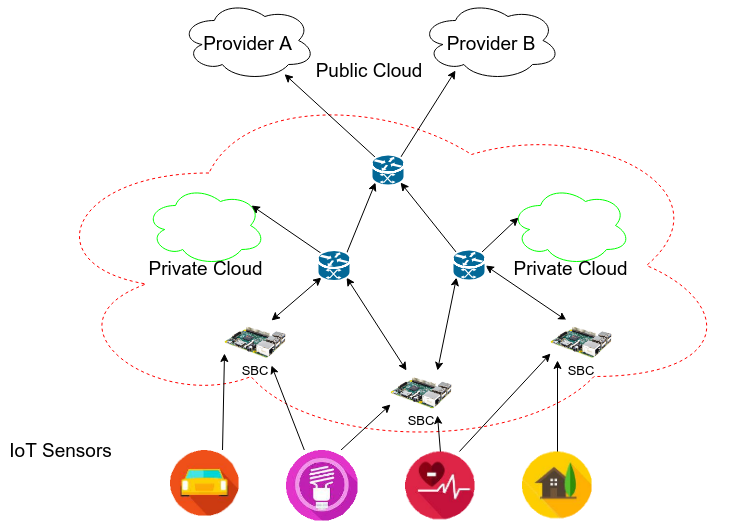
\includegraphics[width=0.4\textwidth]{figures/cassalesimgs-000.png}
%     &
%     asdfasdfa
%     % 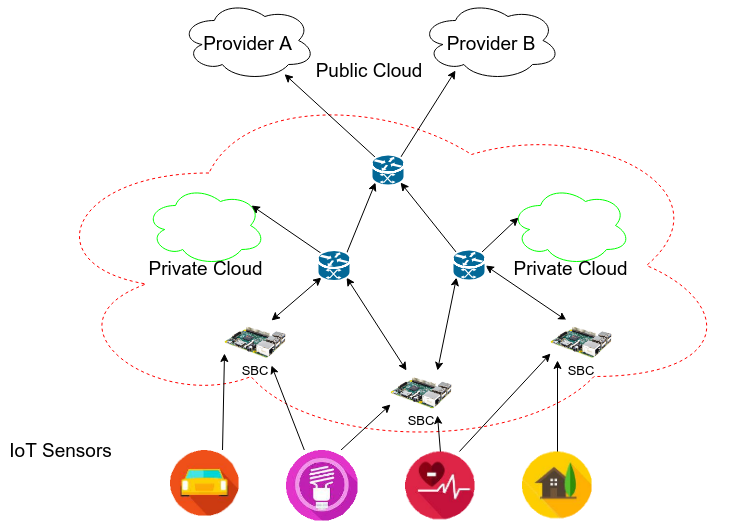
\includegraphics[width=0.4\textwidth]{figures/cassalesimgs-000.png}
% \end{tabular}


% {\begin{algorithm}[h]
% {\tiny 
% \begin{algorithm}
%     \DontPrintSemicolon
%     \SetKwFunction{FMain}{Main}
%     \SetKwProg{Fn}{algorithm}{:}{}
%     \Fn{\FMain{$f$, $a$, $b$, $\varepsilon$}}{
%           a\;
%           b\;
%           \KwRet\;
%     }
%     \;
%     \SetKwProg{Pn}{algorithm}{:}{\KwRet}
%     \Pn{\FMain{$f$, $a$, $b$, $\varepsilon$}}{
%           a\;
%           b\;
%     }
% \end{algorithm}
% \IncMargin{1em}
\begin{algorithm}[h]

% \begin{multicols}{2}
    \SetKwProg{Function}{Function}{:}{}
    % \DontPrintSemicolon
    % \KwIn{sample, ModelSet, params as p}
    % \KwOut{Classified Sample}
    % 
    \SetKwData{CW}{cleaningWindow}
    \SetKwData{NDT}{noveltyDetectionTrigger}
    \SetKwData{MEPC}{minExamplesPerCluster}
    \SetKwData{NF}{noveltyFactor}
    % 
    % \KwSty{Parameters}: cleaningWindow as \CW,
    % noveltyDetectionTrigger as \NDT,
    % minExamplesPerCluster as \MEPC,
    % noveltyFactor as \NF\\
    % 
    \SetKwFunction{nearestCluster}{nearestCluster}
    \SetKwFunction{clustering}{clustering}
    \SetKwFunction{sizeOf}{sizeOf}
    \SetKwFunction{NoveltyDetection}{NoveltyDetection}
    \SetKwFunction{handleModelSleep}{moveToSleep}
    \SetKwFunction{removeOldSamples}{removeOldSamples}
    % 
    % \KwData{ UnkownSet $\leftarrow$ $\emptyset$, ModelSleepSet $\leftarrow$ $\emptyset$, lastCleanupTime $\leftarrow$ now() }
    % 
    \Function{\NoveltyDetection{Model, Samples}}{
        newModelSet $\leftarrow$ $\emptyset$\;
        \ForEach{cl in \clustering(Samples)}{
            \If{$|cl.sampleSet| \geq$ \MEPC}{
                (distance, near) $\leftarrow$ \nearestCluster(cl, Model)\;
                \eIf{distance $<$ near.radius $\times$ \NF}{
                    cl.label $\leftarrow$ near.label\;
                    cl.type $\leftarrow$ extension\;
                }{
                    cl.label $\leftarrow$ noveltyIndex\;
                    noveltyIndex $\leftarrow$ noveltyIndex $+ 1$\;
                    cl.type $\leftarrow$ novelty\;
                }
                Samples $\leftarrow$ Samples $\ominus$ cl.sampleSet\;
                newModelSet $\leftarrow$ newModelSet $\oplus$ cl\;
            }
        }
        \Return{newModelSet}
    }
    \label{alg:MINAS-nd}
    \caption{Minas: Novelty Detection task.}
\end{algorithm}
\begin{algorithm}
    \SetKwProg{function}{Function}{:}{}
    % \DontPrintSemicolon
    % \KwIn{sample, ModelSet, params as p}
    % \KwOut{Classified Sample}
    % 
    \SetKwData{CW}{cleaningWindow}
    \SetKwData{NDT}{noveltyDetectionTrigger}
    \SetKwData{MEPC}{minExamplesPerCluster}
    \SetKwData{NF}{noveltyFactor}
    % 
    % \KwSty{Parameters}: cleaningWindow as \CW,
    % noveltyDetectionTrigger as \NDT,
    % minExamplesPerCluster as \MEPC,
    % noveltyFactor as \NF\\
    % 
    \SetKwFunction{nearestCluster}{nearestCluster}
    \SetKwFunction{clustering}{clustering}
    \SetKwFunction{sizeOf}{sizeOf}
    \SetKwFunction{NoveltyDetection}{NoveltyDetection}
    \SetKwFunction{handleModelSleep}{moveToSleep}
    \SetKwFunction{removeOldSamples}{removeOldSamples}
    % 
    \SetKwProg{algorithm}{algorithm}{:}{}
    \SetKwFor{With}{with}{}{}
    \SetKw{continue}{continue}
    % 
    \SetKwData{CW}{CW}
    \SetKwData{noveltyDetectionTrigger}{NDT}
    \SetKwData{MEPC}{MEPC}
    \SetKwData{NF}{NF}
    \SetKwData{mpiSize}{mpiSize}
    \SetKwData{mpiRank}{mpiRank}
    \SetKwData{EndOfStream}{EndOfStream}
    % 
    \KwIn{ModelSet, Sample Stream}
    \KwOut{Classified Stream as $out$}
    \SetKwFunction{MinasOnline}{MinasOnline}
    \function{\MinasOnline{ModelSet, SampleStream}}{
        UnkownSet $\leftarrow$ $\emptyset$, ModelSleepSet $\leftarrow$ $\emptyset$ \;
        lastCleanup $\leftarrow 0$ , noveltyIndex $\leftarrow 0$\;
        % sampleIn $\leftarrow 0$\;
        \ForEach{ {$sample_{i}$} $\in$ SampleStream }{
            % sample.label $\leftarrow$ unknown\;
            % (distance, cluster) $\leftarrow$ \nearestCluster(sample, ModelSet)\;
            nearest $\leftarrow$ \nearestCluster(sample, ModelSet)\;
            \eIf{nearest.distance $<$ nearest.cluster.radius}{
                sample.label $\leftarrow$ nearest.cluster.label\;
                nearest.cluster.lastUsed $ \leftarrow i $ \;
                % $out \leftarrow$ sample\;
                % outputStream.append(sample);
                % \textbf{continue};
                % \Return sample\;
            }
            {
                sample.label $\leftarrow$ unknown\;
                UnkownSet $\leftarrow$ UnkownSet $\cup$ sample\;
                \If{$|UnkownSet| \geq$ \NDT}{
                    % \tcc{Novelty Detection}
                    novelties $\leftarrow$ \NoveltyDetection(ModelSet $\cup$ ModelSleepSet, *UnkownSet)\;
                    ModelSet $\leftarrow$ ModelSet $\cup$ novelties\;
                }
                \If{ $ i > $ ( lastCleanup $ + $ \CW )}{
                    ModelSet $\leftarrow$ \handleModelSleep(ModelSet, *ModelSleepSet, lastCleanup)\;
                    UnkownSet $\leftarrow$ \removeOldSamples(UnkownSet, lastCleanup)\;
                    lastCleanup $ \leftarrow i $\;
                }
                % \Return sample\;
            }
            outputStream.append(sample);
            % $out \leftarrow$ sample\;
        }
    }
% \end{multicols}
% }
\label{alg:MINAS}
\caption{Our interpretation of MINAS \cite{faria2013novelty,Faria2016minas,Cassales2019a}}
\end{algorithm}
% \DecMargin{1em}


% --------------------------------------------------------------------------------------------------

% \begin{algorithm}[ht]
%   \caption{MINAS \cite{Faria2016minas,Cassales2019a}}
%   \label{alg:MINAS}
%   \renewcommand{\algorithmicrequire}{\textbf{Entrada:}}
%   \begin{algorithmic}[1]
%     %T $\leftarrow$ limiar de distância para pertencer ao grupo
%     %P $\leftarrow$ tempo de "inatividade" para passar para memória sleep
%     %ts $\leftarrow$ limiar para remoção de exemplos da memória temporária
%     \REQUIRE $Modelo,FCD,T,NumMinExemplos,ts,P$
%     \STATE $MemTmp \leftarrow \emptyset$
%     \STATE $MemSleep \leftarrow \emptyset$
%     \FORALL{$exemplo \in FCD$}
%     \STATE $(Dist,micro) \leftarrow$ micro-mais-proximo($exemplo,Modelo$)
%     \IF{$Dist < $ raio($micro$)}
%     \STATE $exemplo.classe \leftarrow micro.rotulo$
%     \STATE atualizar-micro($micro,exemplo$)
%     \ELSE
%     \STATE $exemplo.classe \leftarrow desconhecido$
%     \STATE $MemTmp \leftarrow MemTmp \cup exemplo$
%     \IF{$|MemTmp| \geq NumMinExemplos$}
%     \STATE $Modelo \leftarrow $ deteccao-novidade($Modelo,MemTmp,T$)
%     \ENDIF
%     \ENDIF
%     \STATE $TempoAtual \leftarrow exemplo.T$
%     \IF{$TempoAtual$ mod $TamJanela == 0$}
%     \STATE $Modelo \leftarrow$ mover-micro-grupos-mem-sleep($Modelo,MemSleep,P$)
%     \STATE $MemTmp \leftarrow$ remover-exemplos-antigos($MemTmp,ts$)
%     \ENDIF
%     \ENDFOR
%   \end{algorithmic}
% \end{algorithm}

% \begin{algorithm}[ht]
%   \caption{MINAS \cite{Faria2016minas,Cassales2019a}}
%   \label{alg:MINAS}
%   \renewcommand{\algorithmicrequire}{\textbf{Entrada:}}
%   \begin{algorithmic}[1]
%   \IF{root}
%     \WHILE{true}
%     \IF{can_read(S)}
%     input(S, $s$)
%     send(s, i++)
%     \ENDIF
%     \IF{can_rcv($(s, l)$, any)}
%         output($(s, l)$)
%         \IF{$l == '-'$ )}
%             store($(s, l)$, unknowns)
%             % \IF{$|MemTmp| \geq NumMinExemplos$}
%             % \STATE $Modelo \leftarrow $ deteccao-novidade($Modelo,MemTmp,T$)
%             % \ENDIF
%             % \ENDIF
%             % \STATE $TempoAtual \leftarrow exemplo.T$
%             % \IF{$TempoAtual$ mod $TamJanela == 0$}
%             % \STATE $Modelo \leftarrow$ mover-micro-grupos-mem-sleep($Modelo,MemSleep,P$)
%             % \STATE $MemTmp \leftarrow$ remover-exemplos-antigos($MemTmp,ts$)
%             % \ENDIF
%         \ENDIF
%     \ENDIF
%   \ENDWHILE
%   \ENDIF
%   \IF{leaf}
%     rcv($s$, root)
%     $l$ $\leftarrow$ classify($s$)
%     send($(s, l)$, root)
%   \ENDIF
%   \end{algorithmic}
% \end{algorithm}

% \begin{algorithm}
%   \caption{High level parallel algorithm}
%   \label{alg:highlevel-new}
%   \begin{algorithmic}[1]
%     \State {\bf Input}: an ensemble $E$, $num\_threads$, a data stream $S$
%     \State $P \gets Create\_service\_thread\_pool(num\_threads)$
%     \State $T \gets Create\_trainers\_collection(E)$
%     \For {each arriving instance $I$ in stream $S$}
%     \State $E$.classify($I$)
%     \For  {each trainer $T_i$ in trainers $T$} 
%     \State $k \gets poisson(\lambda)$
%     \State $T_i.update(I, k)$
%     \EndFor
%     \For {all trainers $T$} {\bf in parallel}
%     \State $W\_inst \gets I * k$
%     \State $Train\_on\_instance(W\_inst)$
%     \EndFor
%     \If {change detected}
%     \State $reset\_classifier$
%     \EndIf
%     \EndFor
%   \end{algorithmic}
% \end{algorithm}

 }
% \label{alg:MINAS}
% \caption{Our interpretation of MINAS \cite{faria2013novelty,Faria2016minas,Cassales2019a}}
% \end{algorithm}}

% \begin{figure}[ht]
%     \subfloat[Percentage storage utilization]{
%         \begin{minipage}[c][1\width]{0.4\textwidth}
%         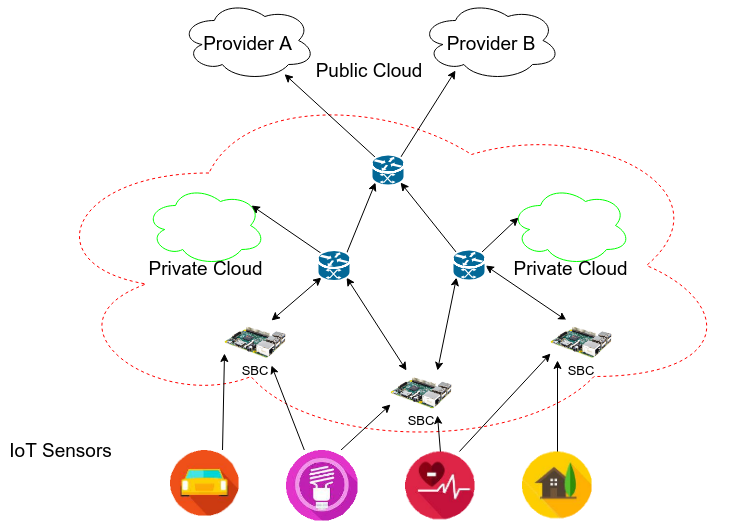
\includegraphics[width=1.1\textwidth]{figures/cassalesimgs-000.png}
%         \end{minipage}}
%     %   \begin{minipage}[c][1\width]{0.5\textwidth}
%     %     %  \includegraphics[width=1\textwidth]{image_file_name}
%     %     \begin{algorithm}[h]
%     %     % {\tiny 
% \begin{algorithm}
%     \DontPrintSemicolon
%     \SetKwFunction{FMain}{Main}
%     \SetKwProg{Fn}{algorithm}{:}{}
%     \Fn{\FMain{$f$, $a$, $b$, $\varepsilon$}}{
%           a\;
%           b\;
%           \KwRet\;
%     }
%     \;
%     \SetKwProg{Pn}{algorithm}{:}{\KwRet}
%     \Pn{\FMain{$f$, $a$, $b$, $\varepsilon$}}{
%           a\;
%           b\;
%     }
% \end{algorithm}
% \IncMargin{1em}
\begin{algorithm}[h]

% \begin{multicols}{2}
    \SetKwProg{Function}{Function}{:}{}
    % \DontPrintSemicolon
    % \KwIn{sample, ModelSet, params as p}
    % \KwOut{Classified Sample}
    % 
    \SetKwData{CW}{cleaningWindow}
    \SetKwData{NDT}{noveltyDetectionTrigger}
    \SetKwData{MEPC}{minExamplesPerCluster}
    \SetKwData{NF}{noveltyFactor}
    % 
    % \KwSty{Parameters}: cleaningWindow as \CW,
    % noveltyDetectionTrigger as \NDT,
    % minExamplesPerCluster as \MEPC,
    % noveltyFactor as \NF\\
    % 
    \SetKwFunction{nearestCluster}{nearestCluster}
    \SetKwFunction{clustering}{clustering}
    \SetKwFunction{sizeOf}{sizeOf}
    \SetKwFunction{NoveltyDetection}{NoveltyDetection}
    \SetKwFunction{handleModelSleep}{moveToSleep}
    \SetKwFunction{removeOldSamples}{removeOldSamples}
    % 
    % \KwData{ UnkownSet $\leftarrow$ $\emptyset$, ModelSleepSet $\leftarrow$ $\emptyset$, lastCleanupTime $\leftarrow$ now() }
    % 
    \Function{\NoveltyDetection{Model, Samples}}{
        newModelSet $\leftarrow$ $\emptyset$\;
        \ForEach{cl in \clustering(Samples)}{
            \If{$|cl.sampleSet| \geq$ \MEPC}{
                (distance, near) $\leftarrow$ \nearestCluster(cl, Model)\;
                \eIf{distance $<$ near.radius $\times$ \NF}{
                    cl.label $\leftarrow$ near.label\;
                    cl.type $\leftarrow$ extension\;
                }{
                    cl.label $\leftarrow$ noveltyIndex\;
                    noveltyIndex $\leftarrow$ noveltyIndex $+ 1$\;
                    cl.type $\leftarrow$ novelty\;
                }
                Samples $\leftarrow$ Samples $\ominus$ cl.sampleSet\;
                newModelSet $\leftarrow$ newModelSet $\oplus$ cl\;
            }
        }
        \Return{newModelSet}
    }
    \label{alg:MINAS-nd}
    \caption{Minas: Novelty Detection task.}
\end{algorithm}
\begin{algorithm}
    \SetKwProg{function}{Function}{:}{}
    % \DontPrintSemicolon
    % \KwIn{sample, ModelSet, params as p}
    % \KwOut{Classified Sample}
    % 
    \SetKwData{CW}{cleaningWindow}
    \SetKwData{NDT}{noveltyDetectionTrigger}
    \SetKwData{MEPC}{minExamplesPerCluster}
    \SetKwData{NF}{noveltyFactor}
    % 
    % \KwSty{Parameters}: cleaningWindow as \CW,
    % noveltyDetectionTrigger as \NDT,
    % minExamplesPerCluster as \MEPC,
    % noveltyFactor as \NF\\
    % 
    \SetKwFunction{nearestCluster}{nearestCluster}
    \SetKwFunction{clustering}{clustering}
    \SetKwFunction{sizeOf}{sizeOf}
    \SetKwFunction{NoveltyDetection}{NoveltyDetection}
    \SetKwFunction{handleModelSleep}{moveToSleep}
    \SetKwFunction{removeOldSamples}{removeOldSamples}
    % 
    \SetKwProg{algorithm}{algorithm}{:}{}
    \SetKwFor{With}{with}{}{}
    \SetKw{continue}{continue}
    % 
    \SetKwData{CW}{CW}
    \SetKwData{noveltyDetectionTrigger}{NDT}
    \SetKwData{MEPC}{MEPC}
    \SetKwData{NF}{NF}
    \SetKwData{mpiSize}{mpiSize}
    \SetKwData{mpiRank}{mpiRank}
    \SetKwData{EndOfStream}{EndOfStream}
    % 
    \KwIn{ModelSet, Sample Stream}
    \KwOut{Classified Stream as $out$}
    \SetKwFunction{MinasOnline}{MinasOnline}
    \function{\MinasOnline{ModelSet, SampleStream}}{
        UnkownSet $\leftarrow$ $\emptyset$, ModelSleepSet $\leftarrow$ $\emptyset$ \;
        lastCleanup $\leftarrow 0$ , noveltyIndex $\leftarrow 0$\;
        % sampleIn $\leftarrow 0$\;
        \ForEach{ {$sample_{i}$} $\in$ SampleStream }{
            % sample.label $\leftarrow$ unknown\;
            % (distance, cluster) $\leftarrow$ \nearestCluster(sample, ModelSet)\;
            nearest $\leftarrow$ \nearestCluster(sample, ModelSet)\;
            \eIf{nearest.distance $<$ nearest.cluster.radius}{
                sample.label $\leftarrow$ nearest.cluster.label\;
                nearest.cluster.lastUsed $ \leftarrow i $ \;
                % $out \leftarrow$ sample\;
                % outputStream.append(sample);
                % \textbf{continue};
                % \Return sample\;
            }
            {
                sample.label $\leftarrow$ unknown\;
                UnkownSet $\leftarrow$ UnkownSet $\cup$ sample\;
                \If{$|UnkownSet| \geq$ \NDT}{
                    % \tcc{Novelty Detection}
                    novelties $\leftarrow$ \NoveltyDetection(ModelSet $\cup$ ModelSleepSet, *UnkownSet)\;
                    ModelSet $\leftarrow$ ModelSet $\cup$ novelties\;
                }
                \If{ $ i > $ ( lastCleanup $ + $ \CW )}{
                    ModelSet $\leftarrow$ \handleModelSleep(ModelSet, *ModelSleepSet, lastCleanup)\;
                    UnkownSet $\leftarrow$ \removeOldSamples(UnkownSet, lastCleanup)\;
                    lastCleanup $ \leftarrow i $\;
                }
                % \Return sample\;
            }
            outputStream.append(sample);
            % $out \leftarrow$ sample\;
        }
    }
% \end{multicols}
% }
\label{alg:MINAS}
\caption{Our interpretation of MINAS \cite{faria2013novelty,Faria2016minas,Cassales2019a}}
\end{algorithm}
% \DecMargin{1em}


% --------------------------------------------------------------------------------------------------

% \begin{algorithm}[ht]
%   \caption{MINAS \cite{Faria2016minas,Cassales2019a}}
%   \label{alg:MINAS}
%   \renewcommand{\algorithmicrequire}{\textbf{Entrada:}}
%   \begin{algorithmic}[1]
%     %T $\leftarrow$ limiar de distância para pertencer ao grupo
%     %P $\leftarrow$ tempo de "inatividade" para passar para memória sleep
%     %ts $\leftarrow$ limiar para remoção de exemplos da memória temporária
%     \REQUIRE $Modelo,FCD,T,NumMinExemplos,ts,P$
%     \STATE $MemTmp \leftarrow \emptyset$
%     \STATE $MemSleep \leftarrow \emptyset$
%     \FORALL{$exemplo \in FCD$}
%     \STATE $(Dist,micro) \leftarrow$ micro-mais-proximo($exemplo,Modelo$)
%     \IF{$Dist < $ raio($micro$)}
%     \STATE $exemplo.classe \leftarrow micro.rotulo$
%     \STATE atualizar-micro($micro,exemplo$)
%     \ELSE
%     \STATE $exemplo.classe \leftarrow desconhecido$
%     \STATE $MemTmp \leftarrow MemTmp \cup exemplo$
%     \IF{$|MemTmp| \geq NumMinExemplos$}
%     \STATE $Modelo \leftarrow $ deteccao-novidade($Modelo,MemTmp,T$)
%     \ENDIF
%     \ENDIF
%     \STATE $TempoAtual \leftarrow exemplo.T$
%     \IF{$TempoAtual$ mod $TamJanela == 0$}
%     \STATE $Modelo \leftarrow$ mover-micro-grupos-mem-sleep($Modelo,MemSleep,P$)
%     \STATE $MemTmp \leftarrow$ remover-exemplos-antigos($MemTmp,ts$)
%     \ENDIF
%     \ENDFOR
%   \end{algorithmic}
% \end{algorithm}

% \begin{algorithm}[ht]
%   \caption{MINAS \cite{Faria2016minas,Cassales2019a}}
%   \label{alg:MINAS}
%   \renewcommand{\algorithmicrequire}{\textbf{Entrada:}}
%   \begin{algorithmic}[1]
%   \IF{root}
%     \WHILE{true}
%     \IF{can_read(S)}
%     input(S, $s$)
%     send(s, i++)
%     \ENDIF
%     \IF{can_rcv($(s, l)$, any)}
%         output($(s, l)$)
%         \IF{$l == '-'$ )}
%             store($(s, l)$, unknowns)
%             % \IF{$|MemTmp| \geq NumMinExemplos$}
%             % \STATE $Modelo \leftarrow $ deteccao-novidade($Modelo,MemTmp,T$)
%             % \ENDIF
%             % \ENDIF
%             % \STATE $TempoAtual \leftarrow exemplo.T$
%             % \IF{$TempoAtual$ mod $TamJanela == 0$}
%             % \STATE $Modelo \leftarrow$ mover-micro-grupos-mem-sleep($Modelo,MemSleep,P$)
%             % \STATE $MemTmp \leftarrow$ remover-exemplos-antigos($MemTmp,ts$)
%             % \ENDIF
%         \ENDIF
%     \ENDIF
%   \ENDWHILE
%   \ENDIF
%   \IF{leaf}
%     rcv($s$, root)
%     $l$ $\leftarrow$ classify($s$)
%     send($(s, l)$, root)
%   \ENDIF
%   \end{algorithmic}
% \end{algorithm}

% \begin{algorithm}
%   \caption{High level parallel algorithm}
%   \label{alg:highlevel-new}
%   \begin{algorithmic}[1]
%     \State {\bf Input}: an ensemble $E$, $num\_threads$, a data stream $S$
%     \State $P \gets Create\_service\_thread\_pool(num\_threads)$
%     \State $T \gets Create\_trainers\_collection(E)$
%     \For {each arriving instance $I$ in stream $S$}
%     \State $E$.classify($I$)
%     \For  {each trainer $T_i$ in trainers $T$} 
%     \State $k \gets poisson(\lambda)$
%     \State $T_i.update(I, k)$
%     \EndFor
%     \For {all trainers $T$} {\bf in parallel}
%     \State $W\_inst \gets I * k$
%     \State $Train\_on\_instance(W\_inst)$
%     \EndFor
%     \If {change detected}
%     \State $reset\_classifier$
%     \EndIf
%     \EndFor
%   \end{algorithmic}
% \end{algorithm}

 }
%     %     \SetAlgoVlined
%     %     \KwIn{sample, ModelSet, params as p}
%     %     \label{alg:MINAS}
%     %     \caption{Our interpretation of MINAS \cite{faria2013novelty,Faria2016minas,Cassales2019a}}
%     %     \end{algorithm}
%     %   \end{minipage}}
%    \hfill
%     \subfloat[standard deviation]{
%       \begin{minipage}[c][1\width]{0.4\textwidth}
%     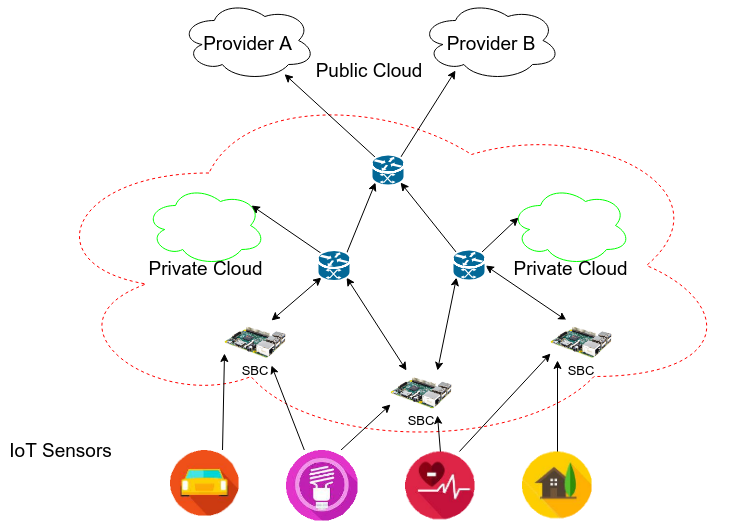
\includegraphics[width=1.1\textwidth]{figures/cassalesimgs-000.png}
%       \end{minipage}}
%   \caption{}
% \end{figure}